\chapter{度量空间上的映射}
\label{chap:metric-space-maps}

测量一个量时总有误差，算出的结果也就带着误差：输入偏差$0.001$时，输出会偏差多少？是不是在某些位置，很小的输入偏差会被放大成很大的输出偏差？用一列简单的函数逼近复杂函数时，逼近函数的连续性能否传给极限？解方程$x=T(x)$时反复代入，迭代何时一定收敛，算到第几步可以停止？这些问题都在研究映射怎样传递距离、极限和误差。第~\ref{chap:topological-spaces}章的连续性只回答“附近的点是否映到附近”，第~\ref{chap:metric-spaces}章的距离则让我们能够回答“误差变成多大”。

本章先把开集原像定义的连续性翻译成距离与点列的判据，再逐步加强为对整个定义域有效的均匀连续与Lipschitz连续。接下来研究一列映射的逐点与一致收敛，以及一族映射共用阈值的等度连续性。然后比较度量空间：等距映射、同胚与同一集合上的几种度量等价，分别保留哪些性质。最后两节把映射条件与完备性结合起来，一是把稠密子集上的均匀连续映射延拓到全空间，二是用压缩映射的迭代求出唯一的不动点并估计误差。

卷一已在实轴区间上讨论过一致连续、Lipschitz连续与函数列的一致收敛，本章把它们放到一般度量空间中，并补充只有在一般空间中才显现的区别。一致度量下的函数空间及其范数结构在第~\ref{chap:normed-spaces}章展开；等度连续函数族的紧性判据与覆盖数估计在第~\ref{chap:function-class-covers}章给出。

\section{连续性的判据}
\label{sec:mmap-continuity-criteria}

第~\ref{chap:topological-spaces}章用开集原像定义了连续映射，也把“在一点$x$连续”写成了邻域的语言：$f(x)$的每个邻域$V$，都对应$x$的某个邻域$U$，使$f(U)\subseteq V$。在度量空间中，邻域可以换成球，这句话就变成输入误差与输出误差之间的一句保证：输出精度要求多高，都能找到足够小的输入误差范围来满足它。

本节先写出这句保证，并证明它与开集定义一致，再用点列来检验连续性。度量空间中点列足以判断连续，一般拓扑空间里却只有单方向的结论，这一差别也放在本节说明。

本章固定记号：$(X,d_X)$与$(Y,d_Y)$是度量空间，$f:X\to Y$是映射；不致混淆时把两个度量都写作$d$。

\subsection{连续性的距离判据}
\label{sec:mmap-epsilon-delta}

先用一个具体函数走一遍。取$f(x)=x^2$，考察$x=1$处的误差。对任何输入$x'$，因式分解给出
\[
 \lvert x'^2-1\rvert=\lvert x'-1\rvert\,\lvert x'+1\rvert.
\]

先约定$\lvert x'-1\rvert<1$，这时$x'\in(0,2)$，第二个因子小于$3$。于是
\[
 \lvert x'^2-1\rvert<3\lvert x'-1\rvert.
\]

要把输出误差控制在$\varepsilon=0.1$以内，只要输入误差小于$0.1/3$。两个要求合起来，取
\[
 \delta=\min\Bigl\{1,\frac{0.1}{3}\Bigr\}=\frac1{30},
\]
则$\lvert x'-1\rvert<\delta$时$\lvert x'^2-1\rvert<0.1$。把$0.1$换成任意$\varepsilon>0$，$\delta=\min\{1,\varepsilon/3\}$同样可用。这就是下面这句保证的一个实例。

图~\ref{fig:mmap-epsilon-delta}把这句保证画成两个球。输出端先给定以$f(x)$为心、半径$\varepsilon$的球，要做的是在输入端找到一个足够小的球$B(x,\delta)$，使它的整个像都落在输出的球内。

\begin{BookInlineFigure}
  \centering
  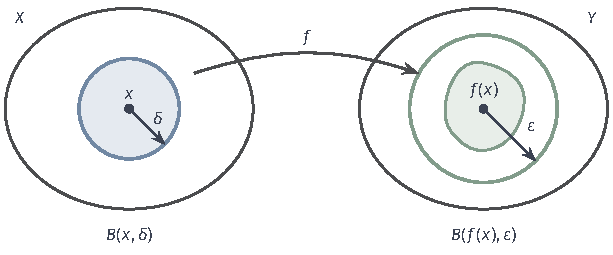
\includegraphics[width=103.738mm]{figures/04-spaces-measures-and-geometry/01-topology-and-metric/tikz/mmap-epsilon-delta/figure.pdf}
  \caption{一点连续的距离判据。蓝色球是输入端的$B(x,\delta)$，绿色圆是输出端的$B(f(x),\varepsilon)$，绿色填充区域是像$f(B(x,\delta))$。给定$\varepsilon$后，要找到足够小的$\delta$，使像完全落在绿色圆内；像本身不必是球。}
  \label{fig:mmap-epsilon-delta}
\end{BookInlineFigure}

把“$f(U)\subseteq V$”中的邻域都换成球，就得到熟悉的$\varepsilon$-$\delta$条件。

\begin{theorem}[一点连续的距离判据]
\label{thm:mmap-epsilon-delta}
$f$在$x\in X$处连续，当且仅当对任意$\varepsilon>0$，存在$\delta>0$，使得对所有$x'\in X$，
\begin{equation}
 d_X(x,x')<\delta
 \quad\Longrightarrow\quad
 d_Y(f(x),f(x'))<\varepsilon.
 \label{eq:mmap-epsilon-delta}
\end{equation}
\end{theorem}

\begin{proof}
设$f$在$x$处连续，给定$\varepsilon>0$。球$B(f(x),\varepsilon)$是$f(x)$的邻域，按一点连续的定义，有$x$的邻域$U$使
\[
 f(U)\subseteq B(f(x),\varepsilon).
\]
度量空间中$x$的邻域包含某个球，设$B(x,\delta)\subseteq U$。这个$\delta$满足式~\eqref{eq:mmap-epsilon-delta}。

反过来，设距离条件成立，$V$是$f(x)$的邻域。$V$包含某个球$B(f(x),\varepsilon)$，对这个$\varepsilon$取条件中的$\delta$，令$U=B(x,\delta)$。则$U$是$x$的邻域，并且
\[
 f(U)\subseteq B(f(x),\varepsilon)\subseteq V.
\]
所以$f$在$x$处连续。
\end{proof}

条件中的$\delta$可以依赖$x$，也可以依赖$\varepsilon$。它回答的问题是：输出允许的误差已经给定，输入需要控制在多小的范围内。前面的$x^2$例子里，$x=1$时用的是$\delta=\min\{1,\varepsilon/3\}$，换到别的点，这个公式就要跟着改变。

下一个定理说明，每一点都满足这句保证，恰好就是第~\ref{chap:topological-spaces}章定义的连续映射。

\begin{theorem}[逐点连续与开集原像]
\label{thm:mmap-pointwise-open-preimage}
$f$在$X$的每一点满足定理~\ref{thm:mmap-epsilon-delta}的距离条件，当且仅当$Y$中每个开集的原像都是$X$中的开集。
\end{theorem}

\begin{proof}
设距离条件处处成立，$U\subseteq Y$是开集，$x\in f^{-1}(U)$。$U$是开集，所以可取$\varepsilon>0$使$B(f(x),\varepsilon)\subseteq U$。再取对应的$\delta$，距离条件给出
\[
 f(B(x,\delta))\subseteq B(f(x),\varepsilon)\subseteq U,
\]
也就是$B(x,\delta)\subseteq f^{-1}(U)$。$x$是$f^{-1}(U)$中任意一点，所以$f^{-1}(U)$是开集。

反过来，设开集的原像都是开集。对$x\in X$和$\varepsilon>0$，集合$f^{-1}(B(f(x),\varepsilon))$是包含$x$的开集，所以其中有某个球$B(x,\delta)$。这个$\delta$满足式~\eqref{eq:mmap-epsilon-delta}。
\end{proof}

由$f^{-1}(Y\setminus F)=X\setminus f^{-1}(F)$，开集原像为开集等价于闭集原像为闭集，后者常用来判断集合是闭集。例如$g(\bm x)=x_1^2+x_2^2$在$(\mathbb R^2,d_2)$上连续，于是单位圆周是闭集，原因是
\[
 S^1=g^{-1}(\{1\}),
\]
单点集$\{1\}$是$\mathbb R$中的闭集；同样，圆盘$\{\bm x:g(\bm x)\leq4\}=g^{-1}((-\infty,4])$也是闭集。

连续性只保证原像保持开闭，不保证像保持开闭。$f(x)=x^2$把开区间$(-1,1)$映成$[0,1)$，后者在$\mathbb R$中不是开集，因为$0$处没有向左的邻域。$f(x)=e^x$把闭集$\mathbb R$映成$(0,\infty)$，后者不是闭集，因为$0$在它的闭包中。把开集映成开集的映射称为开映射，这是另一回事。

距离函数是最常用的连续函数。固定$z\in X$，由三角不等式$d(x,z)\leq d(x,x')+d(x',z)$，交换$x,x'$后合起来得到
\[
 \lvert d(x,z)-d(x',z)\rvert\leq d(x,x').
\]

对非空集合$A\subseteq X$，每个$a\in A$满足$d(x,A)\leq d(x,a)\leq d(x,x')+d(x',a)$。对$a$取下确界，再交换$x,x'$，得到
\[
 \lvert d(x,A)-d(x',A)\rvert\leq d(x,x').
\]

这两个函数都可以取$\delta=\varepsilon$，并且这个$\delta$对所有点通用，这种通用性下一节将命名为均匀连续。它们的零点集分别是$\{z\}$和$\overline A$，这再次说明单点集与闭包都是闭集。

\subsection{连续性的序列判据}
\label{sec:mmap-sequential-continuity}

对每个$\varepsilon$找$\delta$，有时不如直接看点列方便。上一章已经用点列描述了闭包，度量空间中点列同样足以探测连续性。

\begin{theorem}[连续性的序列判据]
\label{thm:mmap-sequential-continuity}
$f$在$x$处连续，当且仅当对$X$中每个满足$x_n\to x$的点列，都有$f(x_n)\to f(x)$。
\end{theorem}

\begin{proof}
设$f$在$x$处连续，$x_n\to x$。给定$\varepsilon>0$，取距离条件中的$\delta$，再取$N$使$n\geq N$时$d(x_n,x)<\delta$。这些$n$都满足
\[
 d(f(x_n),f(x))<\varepsilon,
\]
所以$f(x_n)\to f(x)$。

反方向用反证法。设$f$在$x$处不连续，按定理~\ref{thm:mmap-epsilon-delta}，存在某个$\varepsilon>0$，使任何$\delta>0$都不满足条件。对每个$n$取$\delta=1/n$，这一失败给出一点$x_n$，满足
\[
 d(x_n,x)<\frac1n,\qquad d(f(x_n),f(x))\geq\varepsilon.
\]
于是$x_n\to x$，而$f(x_n)$不趋于$f(x)$，与假设矛盾。
\end{proof}

序列判据特别适合否定连续性：只需找到一个趋于$x$、像却不趋于$f(x)$的点列。在$\mathbb R^2$上令
\[
 f(\bm x)=\frac{x_1x_2}{x_1^2+x_2^2}\quad(\bm x\neq\bm 0),\qquad f(\bm 0)=0.
\]

沿对角线上的点$\bm x_n=(1/n,1/n)$，分子是$1/n^2$，分母是$2/n^2$，于是
\[
 f(\bm x_n)=\frac12,\qquad \bm x_n\to\bm 0,
\]
像不趋于$f(\bm 0)=0$，所以$f$在原点不连续。沿坐标轴趋近时函数值恒为$0$，只看这个方向会得出错误结论：判据要求每一个趋于该点的点列都保持极限。

序列判据也可以用来肯定连续性。设$f:X\to Y$在$x$处连续，$g:Y\to Z$在$f(x)$处连续。若$x_n\to x$，则$f(x_n)\to f(x)$，再由$g$的连续性得
\[
 g(f(x_n))\to g(f(x)).
\]
所以$g\circ f$在$x$处连续。第~\ref{chap:topological-spaces}章已用开集原像证明了复合映射的连续性，这里是它在度量空间中的另一种读法。

在一般拓扑空间中，正方向仍然成立。若$f$连续且$x_n\to x$，对$f(x)$的邻域$V$，$f^{-1}(V)$是$x$的邻域，点列最终落在其中，所以$f(x_n)$最终落在$V$中。

反方向依赖于点列能否探测拓扑。上面的证明取$\delta=1/n$依次选点，用的正是每点有可数个球作邻域基；第~\ref{chap:topological-spaces}章的余可数拓扑没有这样的邻域基，那里给出了保持全部收敛点列、却不连续的映射。

\section{均匀连续与Lipschitz连续}
\label{sec:mmap-uniform-lipschitz}

连续性允许$\delta$随输入点改变。处理单个点附近的问题时这无关紧要，但处理柯西列、稠密集上的延拓或迭代误差时，点列的各项散布在不同位置，需要一个对整个定义域都有效的阈值，最好还能给出输出误差是输入误差的多少倍。本节依次加强条件：均匀连续要求阈值与位置无关，Lipschitz连续要求误差按固定比例放大。最后说明紧定义域上连续自动升级为均匀连续，却不能自动升级为Lipschitz连续。卷一在实轴区间上讨论过这些概念，可参考\BookChapterRef{chap:limits-continuity}{卷一“极限与连续”章}，这里推广到度量空间。

\subsection{均匀连续}
\label{sec:mmap-uniform-continuity}

先看阈值怎样依赖位置。在$\mathbb R$上取$f(x)=x^2$，有$\lvert f(x')-f(x)\rvert=\lvert x'-x\rvert\,\lvert x'+x\rvert$。在$x$附近要使输出误差小于$1$，输入误差大约要小于$1/(2\lvert x\rvert)$，$x$越大，允许的输入误差越小。换到区间$[0,1]$上，$\lvert x'+x\rvert\leq2$，于是$\lvert f(x')-f(x)\rvert\leq2\lvert x'-x\rvert$，取$\delta=\varepsilon/2$对区间中所有点都有效。

\begin{definition}[均匀连续]
\label{def:mmap-uniform-continuity}
若对任意$\varepsilon>0$，存在$\delta>0$，使得对所有满足$d_X(x,x')<\delta$的$x,x'\in X$，都有$d_Y(f(x),f(x'))<\varepsilon$，则称$f$\term{均匀连续}（uniformly continuous）。卷一称之为一致连续。
\end{definition}

与逐点连续相比，变化只在量词的次序：逐点连续是“对每个$x$和$\varepsilon$，存在$\delta$”，均匀连续是“对每个$\varepsilon$，存在$\delta$，对所有$x,x'$”。否定均匀连续时，常用点对序列：若存在$\varepsilon>0$及点列$x_n,x_n'$，使$d(x_n,x_n')\to0$而$d(f(x_n),f(x_n'))\geq\varepsilon$，则$f$不均匀连续，因为任何$\delta$都会被某个$d(x_n,x_n')<\delta$的点对打破。对$\mathbb R$上的$x^2$，取$x_n=n$，$x_n'=n+1/n$，则$\lvert x_n-x_n'\rvert=1/n\to0$，而$\lvert x_n'^2-x_n^2\rvert=2+1/n^2\geq2$。

均匀连续的直接用处是保持柯西列。

\begin{theorem}[均匀连续映射保持柯西列]
\label{thm:mmap-uniform-cauchy-image}
若$f$均匀连续，$(x_n)$是$X$中的柯西列，则$(f(x_n))$是$Y$中的柯西列。
\end{theorem}

\begin{proof}
对$\varepsilon>0$取均匀连续的$\delta$，再取$N$使$m,n\geq N$时$d(x_m,x_n)<\delta$，则这些$m,n$满足$d(f(x_m),f(x_n))<\varepsilon$。
\end{proof}

仅有连续性不够。$f(x)=1/x$在$(0,1)$上连续，$x_n=1/(n+1)$是柯西列，像$n+1$却不是柯西列；按定理，这也说明$1/x$在$(0,1)$上不均匀连续。第~\ref{sec:mmap-extension}节把均匀连续映射从稠密子集延拓出去，依靠的正是这一定理：逼近同一点的柯西列，其像也是柯西列。

\subsection{Lipschitz连续}
\label{sec:mmap-lipschitz}

均匀连续只说存在$\delta$，没有说$\delta$与$\varepsilon$的关系。若输出误差不超过输入误差的固定倍数，误差估计就可以直接写出来。

\begin{definition}[Lipschitz连续]
\label{def:mmap-lipschitz}
若存在有限常数$L\geq0$，使对所有$x,x'\in X$有
\begin{equation}
d_Y(f(x),f(x'))\leq L\,d_X(x,x'),
\label{eq:mmap-lipschitz}
\end{equation}
则称$f$为\term{Lipschitz连续}（Lipschitz continuous）的，$L$称为一个Lipschitz常数。满足式\eqref{eq:mmap-lipschitz}的最小常数记为
\begin{equation*}
\operatorname{Lip}(f)=\sup_{x\neq x'}\frac{d_Y(f(x),f(x'))}{d_X(x,x')},
\end{equation*}
称为$f$的\term{Lipschitz常数}（Lipschitz constant）。
\end{definition}

Lipschitz连续蕴含均匀连续：$L>0$时取$\delta=\varepsilon/L$，$L=0$时$f$为常值。它还给出可以计算的误差放大界：输入误差为$\eta$时，输出误差至多为$L\eta$。若$f:X\to Y$与$g:Y\to Z$都Lipschitz连续，则
\begin{equation*}
d(g(f(x)),g(f(x')))\leq\operatorname{Lip}(g)\,d(f(x),f(x'))\leq\operatorname{Lip}(g)\operatorname{Lip}(f)\,d(x,x'),
\end{equation*}
所以$\operatorname{Lip}(g\circ f)\leq\operatorname{Lip}(g)\operatorname{Lip}(f)$：多步计算的误差放大倍数至多相乘。

常见的Lipschitz映射有几类。距离函数$x\mapsto d(x,A)$的Lipschitz常数不超过$1$。区间上可微且$\lvert f'\rvert\leq L$的实函数满足$\lvert f(x)-f(x')\rvert=\lvert f'(\xi)\rvert\,\lvert x-x'\rvert\leq L\lvert x-x'\rvert$，这里用到中值定理，可参考\BookChapterRef{chap:univariate-differentiation}{卷一“一元函数的微分”章}；前面的$x^2$在$[0,1]$上就有$L=2$。矩阵$\bm A$定义的线性映射满足$\lVert\bm A\bm x-\bm A\bm y\rVert\leq\lVert\bm A\rVert\,\lVert\bm x-\bm y\rVert$，其中$\lVert\bm A\rVert$是诱导的算子范数，可参考\BookChapterRef{chap:normed-inner-product-spaces}{卷二“赋范空间与内积空间”章}。

均匀连续不必Lipschitz连续。在$[0,1]$上取$f(x)=\sqrt x$。对$0\leq y\leq x$，$(\sqrt y+\sqrt{x-y})^2=x+2\sqrt{y(x-y)}\geq x$，所以$\sqrt x-\sqrt y\leq\sqrt{x-y}$，取$\delta=\varepsilon^2$即得均匀连续。但$\sqrt x/x=1/\sqrt x$在$x\to0^+$时无界，没有有限的$L$满足$\sqrt x-\sqrt0\leq Lx$。平方根在$0$附近把输入误差$\eta$放大为$\sqrt\eta$，放大倍数$1/\sqrt\eta$没有上界。

$L<1$的自映射把任意两点的距离按固定比例缩小，这是第~\ref{sec:mmap-contraction}节压缩迭代的出发点。

\subsection{紧空间上的均匀连续性}
\label{sec:mmap-compact-uniform}

前面的反例$x^2$与$1/x$分别定义在无界的$\mathbb R$和不包含端点的$(0,1)$上，都不是紧空间。紧性恰好排除了阈值随位置无限缩小的情形。

\begin{theorem}[紧空间上的均匀连续性]
\label{thm:mmap-compact-uniform}
若$X$是紧致度量空间，$f:X\to Y$连续，则$f$均匀连续。
\end{theorem}

\begin{proof}
若不然，存在$\varepsilon>0$及点列$x_n,x_n'$，使$d(x_n,x_n')<1/n$而$d(f(x_n),f(x_n'))\geq\varepsilon$。按第~\ref{chap:metric-spaces}章，紧致度量空间序列紧致，取子列$x_{n_k}\to x\in X$，则$d(x'_{n_k},x)\leq d(x'_{n_k},x_{n_k})+d(x_{n_k},x)\to0$。由$f$在$x$处连续及序列判据，$f(x_{n_k})$与$f(x'_{n_k})$都趋于$f(x)$，于是$d(f(x_{n_k}),f(x'_{n_k}))\to0$，与$\geq\varepsilon$矛盾。
\end{proof}

也可以用开覆盖证明：对每个$x$取使$f(B(x,\delta_x))\subseteq B(f(x),\varepsilon/2)$的$\delta_x$，球族$\{B(x,\delta_x)\}$的Lebesgue数就是对全空间通用的阈值。两种证明都把逐点的阈值变成有限个或一个收敛子列能控制的情形。

紧性是充分条件，不是必要条件：恒等映射在$\mathbb R$上均匀连续，而$\mathbb R$不紧。定理也只给出统一的阈值，不给出Lipschitz常数。$[0,1]$紧致，$\sqrt x$在其上连续因而均匀连续，但上一小节已说明它不Lipschitz连续。均匀连续保证存在随$\varepsilon$变化的$\delta(\varepsilon)$，Lipschitz连续则要求$\delta$可以取成$\varepsilon$的固定倍数。

\section{映射列的收敛}
\label{sec:mmap-map-sequences}

用多项式、截断级数或迭代格式逼近一个映射时，得到的是一列映射$f_1,f_2,\ldots$。说它们“趋于”$f$，可以只要求每个固定输入处的输出趋于$f$的值，也可以要求同一个序号对全部输入都达到给定精度。两种要求的差别决定了极限能否继承连续性。本节设$X$是集合（讨论连续性时是拓扑空间），$(Y,d)$是度量空间，$f_n,f:X\to Y$。先定义两种收敛并说明一致距离的适用范围，再证明一致极限保持连续，最后说明目标空间完备时，一致柯西列必有一致极限。

\subsection{逐点收敛与一致收敛}
\label{sec:mmap-pointwise-uniform}

两种收敛的区别在于“达到精度所需的序号”是否允许随输入改变。

\begin{definition}[逐点收敛与一致收敛]
\label{def:mmap-pointwise-uniform}
若对每个$x\in X$，当$n\to\infty$时都有$d(f_n(x),f(x))\to0$，即对每个$x$和$\varepsilon>0$存在$N$（可依赖于$x$）使$n\geq N$时$d(f_n(x),f(x))<\varepsilon$，则称$(f_n)$\term{逐点收敛}（pointwise convergence）于$f$。若对每个$\varepsilon>0$存在不依赖于$x$的$N$，使$n\geq N$时对所有$x\in X$都有$d(f_n(x),f(x))<\varepsilon$，则称$(f_n)$\term{一致收敛}（uniform convergence）于$f$。
\end{definition}

在$[0,1]$上取$f_n(x)=x^n$。对$x\in[0,1)$有$x^n\to0$，而$f_n(1)=1$，所以逐点极限是$f(x)=0$（$x<1$）、$f(1)=1$。所需序号随$x$变化：要使$x^n<0.01$，$x=0.9$时需要$n\geq44$，因为$\ln0.01/\ln0.9\approx43.7$；$x=0.99$时需要$n\geq459$，因为$\ln0.01/\ln0.99\approx458.2$。越接近$1$，所需序号越大，没有一个$N$对全部$x\in[0,1)$有效：对任何$n$，$\sup_{0\leq x<1}x^n=1$。所以这个映射列不一致收敛。限制到$[0,1/2]$上，$\sup_{0\leq x\leq1/2}x^n=2^{-n}\to0$，就一致收敛于$0$。

一致收敛可以用一个量来概括。令
\begin{equation}
d_\infty(f,g)=\sup_{x\in X}d(f(x),g(x))\in[0,\infty],
\label{eq:mmap-uniform-distance}
\end{equation}
则$f_n$一致收敛于$f$当且仅当$d_\infty(f_n,f)\to0$。但$d_\infty$可能取值$\infty$：在$\mathbb R$上，$f(x)=x$与$g(x)=0$的上确界距离是$\infty$。因此它不能在全体映射上当作通常的度量。

把映射限制在像集有界的映射上，问题就消失了。若$f(X)$含于$Y$的某个球，称$f$为\term{有界映射}（bounded map），记全体有界映射为$B(X,Y)$。对$f,g\in B(X,Y)$，$f(X)\subseteq B(y_1,r_1)$、$g(X)\subseteq B(y_2,r_2)$，则$d(f(x),g(x))<r_1+d(y_1,y_2)+r_2$，所以$d_\infty(f,g)<\infty$。三角不等式逐点成立再取上确界，$d_\infty(f,h)\leq d_\infty(f,g)+d_\infty(g,h)$，零距离判定也逐点成立，所以$d_\infty$是$B(X,Y)$上的度量，称为\term{一致度量}（uniform metric）。在一般映射上谈一致收敛时，仍然使用定义~\ref{def:mmap-pointwise-uniform}的$\varepsilon$-$N$表述，只要求$d_\infty(f_n,f)$最终有限并趋于零。

\subsection{一致极限的连续性}
\label{sec:mmap-uniform-limit-continuity}

$x^n$的例子中，每个$f_n$都连续，逐点极限却在$x=1$处跳跃。一致收敛排除了这种情形，证明只需把误差分成三段。

\begin{theorem}[一致极限保持连续]
\label{thm:mmap-uniform-limit-continuous}
设$X$是拓扑空间，$(Y,d)$是度量空间，$f_n:X\to Y$连续，并且一致收敛于$f$。则$f$连续。
\end{theorem}

\begin{proof}
设$V\subseteq Y$是开集，$x\in f^{-1}(V)$。取$\varepsilon>0$使$B(f(x),\varepsilon)\subseteq V$，再取$N$使对所有$x'\in X$都有$d(f_N(x'),f(x'))<\varepsilon/3$。$f_N$连续，所以$U=f_N^{-1}\bigl(B(f_N(x),\varepsilon/3)\bigr)$是含$x$的开集。对$x'\in U$，
\begin{equation*}
\begin{aligned}
d(f(x'),f(x))
&\leq d(f(x'),f_N(x'))+d(f_N(x'),f_N(x))+d(f_N(x),f(x))\\
&<\tfrac\varepsilon3+\tfrac\varepsilon3+\tfrac\varepsilon3=\varepsilon,
\end{aligned}
\end{equation*}
所以$U\subseteq f^{-1}(V)$。$f^{-1}(V)$的每个点都有含于其中的开集，它是开集。
\end{proof}

三段误差中，首尾两段由一致收敛控制，并且用的是同一个$N$；中间一段由单个$f_N$的连续性控制。若只有逐点收敛，首段$d(f(x'),f_N(x'))$所需的$N$随$x'$变化，无法与中间一段的邻域$U$同时取定，$x^n$正是这样失败的。

定理的条件很少：定义域只需是拓扑空间，不要求紧致；目标空间只需是度量空间，不要求完备，因为极限$f$已经假定存在。一致收敛也只是充分条件：$x^n$在$[0,1)$上逐点收敛于连续函数$0$，但不一致收敛。

\subsection{一致柯西列的极限}
\label{sec:mmap-uniform-cauchy}

上一小节假定了极限$f$存在。和点列一样，实际中往往只能看到映射列的后项彼此接近，需要从这一点推出极限存在。

\begin{definition}[一致柯西列]
\label{def:mmap-uniform-cauchy}
若对任意$\varepsilon>0$，存在$N$，使$m,n\geq N$时对所有$x\in X$都有$d(f_m(x),f_n(x))<\varepsilon$，则称$(f_n)$为\term{一致柯西列}（uniformly Cauchy sequence）。
\end{definition}

\begin{theorem}[一致柯西列的一致极限]
\label{thm:mmap-uniform-cauchy-limit}
设$(Y,d)$完备，$(f_n)$是$X\to Y$的一致柯西列。则存在$f:X\to Y$，使$f_n$一致收敛于$f$。
\end{theorem}

\begin{proof}
对每个固定的$x$，$(f_n(x))$是$Y$中的柯西列，由完备性收敛，记极限为$f(x)$。给定$\varepsilon>0$，取$N$使$m,n\geq N$时对所有$x$有$d(f_n(x),f_m(x))<\varepsilon$。固定$n\geq N$和$x$，令$m\to\infty$。由第~\ref{chap:metric-spaces}章的不等式$\lvert d(a,b)-d(a,c)\rvert\leq d(b,c)$，$d(f_n(x),f_m(x))\to d(f_n(x),f(x))$，所以$d(f_n(x),f(x))\leq\varepsilon$。这对所有$x$和所有$n\geq N$成立，即一致收敛。
\end{proof}

证明的顺序值得注意：先逐点取极限得到候选的$f$，再在不等式中让后项趋于极限，把对所有$x$统一的估计传给$f$。目标空间的完备性不可省略。取$Y=\mathbb Q$，$f_n$为常值映射，取值为$\sqrt2$的第$n$个十进制截断，它们是一致柯西列，却没有取值在$\mathbb Q$中的极限。

把本小节与上一小节合起来，就得到函数空间完备性的共同依据。

\begin{theorem}[有界映射空间的完备性]
\label{thm:mmap-bounded-maps-complete}
设$(Y,d)$完备。则$(B(X,Y),d_\infty)$完备。若$X$是拓扑空间，有界连续映射全体$C_b(X,Y)$是$B(X,Y)$的闭子集，因而也完备。
\end{theorem}

\begin{proof}
$B(X,Y)$中关于$d_\infty$的柯西列就是一致柯西列，由定理~\ref{thm:mmap-uniform-cauchy-limit}一致收敛于某个$f$。取$N$使$d_\infty(f_N,f)\leq1$，$f_N$的像含于某个球$B(y,r)$，则$f$的像含于$B(y,r+1)$，$f\in B(X,Y)$，并且$d_\infty(f_n,f)\to0$。若各$f_n$还连续，由定理~\ref{thm:mmap-uniform-limit-continuous}，$f$连续。这说明$C_b(X,Y)$包含其中点列的极限，是闭集；按第~\ref{chap:metric-spaces}章，完备空间的闭子空间完备。
\end{proof}

$X$紧致时，连续映射的像是紧集，因而有界，所以$C_b(X,Y)$就是全体连续映射$C(X,Y)$。例如$C([0,1],\mathbb R)$在一致度量下完备。检验具体的函数列时，常常先估计一致柯西性。在$[0,1]$上令$s_n(x)=\sum_{k=1}^nx^k/k^2$。对$m>n$，
\begin{equation*}
\lvert s_m(x)-s_n(x)\rvert\leq\sum_{k=n+1}^m\frac1{k^2}\leq\sum_{k=n+1}^m\Bigl(\frac1{k-1}-\frac1k\Bigr)<\frac1n,
\end{equation*}
上界与$x$无关，所以$(s_n)$是一致柯西列，一致收敛于一个连续函数。第~\ref{chap:normed-spaces}章核验具体函数空间的完备性时，反复使用的就是这一模式：先逐点取极限，再证明极限属于所考察的空间。

\section{等度连续性}
\label{sec:mmap-equicontinuity}

上一节研究的是一列映射趋于一个极限；有时我们关心的是一整族映射作为整体有多“规整”。例如一族函数各自连续，但随着下标增大越来越陡，它们在同一个输入点附近需要的阈值就越来越小。

均匀连续说的是$\delta$与位置无关，等度连续把这个想法换成$\delta$与族中的成员无关。本节给出定义，并证明在紧定义域上，两种“无关”可以同时实现。

\paragraph{等度连续的定义}
在$[0,1]$上看映射族$\mathcal F=\{x^n:n\geq1\}$，每个$x^n$都连续。先看$x_0=1$，取$\varepsilon=1/2$。对任何$\delta\in(0,1)$，令$x=1-\delta/2$，则$\lvert x-1\rvert<\delta$，而$(1-\delta/2)^n\to0$，所以$n$充分大时
\[
 \lvert x^n-1^n\rvert>\frac12.
\]
没有一个$\delta$对全族有效。

在$x_0=1/2$处情况不同，这里可以把全族分成两组来处理。取$\varepsilon=1/10$，先限制$\lvert x-1/2\rvert<1/4$，此时$x<3/4$，于是
\[
 \lvert x^n-(1/2)^n\rvert\leq(3/4)^n.
\]
由$(3/4)^9\approx0.075$，$n\geq9$的成员在这个半径上已经满足要求。

剩下$n=1,\ldots,8$这八个成员，用中值定理估计。对$x,x'\in[0,3/4]$，
\[
 \lvert x^n-x'^n\rvert\leq n(3/4)^{n-1}\lvert x-x'\rvert\leq\frac{27}{16}\lvert x-x'\rvert,
\]
这里系数$n(3/4)^{n-1}$在$n=3,4$处取最大值$27/16=1.6875$。

要使右端小于$1/10$，只需$\lvert x-x'\rvert<8/135$，于是全族共用的半径可以取
\[
 \delta=\frac1{17}.
\]
验算：$1/17<8/135$，并且$1/17<1/4$，所以这个$\delta$对全部$n$都有效。

\begin{definition}[等度连续]
\label{def:mmap-equicontinuous}
设$\mathcal F$是一族映射$X\to Y$，$x\in X$。若对任意$\varepsilon>0$，存在$\delta>0$，使得对所有$f\in\mathcal F$和所有$x'\in X$，
\begin{equation}
 d(x,x')<\delta
 \quad\Longrightarrow\quad
 d(f(x),f(x'))<\varepsilon,
 \label{eq:mmap-equicontinuous}
\end{equation}
则称$\mathcal F$在$x$处\term{等度连续}（equicontinuous）。若$\mathcal F$在$X$的每一点等度连续，称$\mathcal F$在$X$上等度连续。若$\delta$还可以对所有$x$通用，称$\mathcal F$\term{一致等度连续}（uniformly equicontinuous）。
\end{definition}

上面的$\{x^n\}$在每个$x_0\in[0,1)$处等度连续：取$\delta_0=(1-x_0)/2$，$B(x_0,\delta_0)$内的点都不超过$r=(1+x_0)/2<1$，$r^n$最终小于$\varepsilon$，前面有限个成员再各取一个半径，与$\delta_0$取最小值即可。在$x_0=1$处不等度连续。

每个成员连续，只说明每个$f$都有自己的$\delta_f$；等度连续要求这些$\delta_f$有正的下界。有限族总是满足这一点，取有限个$\delta_f$的最小值就行；无限族则可能不满足，下面的例子把两种情形并排放在一起。

\paragraph{等度连续的例子}
共同的Lipschitz常数给出最简单的等度连续族。若每个$f\in\mathcal F$都满足$d(f(x),f(x'))\leq Ld(x,x')$，取$\delta=\varepsilon/L$，它对所有成员和所有点都有效，所以族一致等度连续。例如平移族$\{x\mapsto\sin(x+c):c\in\mathbb R\}$，每个成员的导数绝对值不超过$1$，是$1$-Lipschitz族。

频率不断增大的族则不然。$\{x\mapsto\sin(nx):n\geq1\}$在$0$处不等度连续：对任何$\delta>0$，取$n>\pi/(2\delta)$，点$x'=\pi/(2n)$满足$\lvert x'\rvert<\delta$，而
\[
 \lvert\sin(nx')-\sin0\rvert=1.
\]

图~\ref{fig:mmap-equicontinuity}并排画出这两族。左边的曲线在宽度$\delta$的窗口内一起缓慢变化，右边的曲线随$n$增大越来越早地冲到$1$，无论窗口多窄，总有成员在窗口内完成一次满振幅。

\begin{BookInlineFigure}
  \centering
  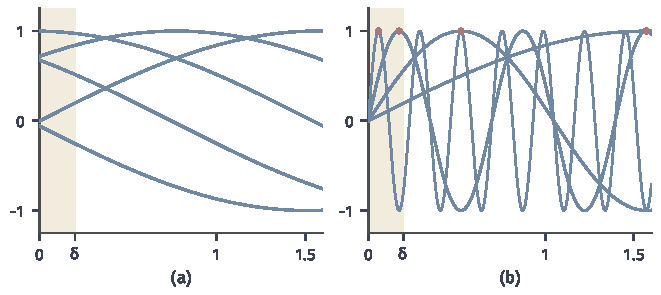
\includegraphics[width=112mm]{figures/04-spaces-measures-and-geometry/01-topology-and-metric/matplotlib/mmap-equicontinuity/figure.pdf}
  \caption{等度连续与不等度连续。(a) 平移族$\sin(x+c)$，$c=0,0.8,1.6,2.4,3.2$，导数绝对值不超过$1$，在宽度$\delta=0.2$的窗口（黄色）内每条曲线的变化不超过$0.2$。(b) $\sin(nx)$，$n=1,3,9,27$，红点是首次到达$1$的位置$x=\pi/(2n)$，当$n$足够大时落进任何给定的窗口。}
  \label{fig:mmap-equicontinuity}
\end{BookInlineFigure}

\paragraph{紧定义域上的统一半径}
均匀连续与连续之间的关系，对映射族同样成立：在紧定义域上，逐点的等度连续可以升级为一致的等度连续。

\begin{theorem}[紧空间上的一致等度连续]
\label{thm:mmap-compact-uniform-equicontinuous}
设$X$是紧致度量空间，$\mathcal F$是在$X$上等度连续的映射族。则$\mathcal F$一致等度连续。
\end{theorem}

\begin{proof}
反证。若结论不成立，存在$\varepsilon>0$，以及$f_n\in\mathcal F$和点列$x_n,x_n'$，使
\[
 d(x_n,x_n')<\frac1n,\qquad d(f_n(x_n),f_n(x_n'))\geq\varepsilon.
\]

由序列紧致性，取子列$x_{n_k}\to x\in X$，由三角不等式，$x'_{n_k}$也趋于$x$。在$x$处用等度连续，取对应于$\varepsilon/2$的$\delta$。

当$k$充分大时，$x_{n_k}$与$x'_{n_k}$都落在$B(x,\delta)$中，于是由三角不等式，
\[
 \begin{aligned}
 d(f_{n_k}(x_{n_k}),f_{n_k}(x'_{n_k}))
 &\leq d(f_{n_k}(x_{n_k}),f_{n_k}(x))\\
 &\quad+d(f_{n_k}(x),f_{n_k}(x'_{n_k}))<\varepsilon.
 \end{aligned}
\]
这与不小于$\varepsilon$矛盾。
\end{proof}

证明与定理~\ref{thm:mmap-compact-uniform}几乎相同，区别只在于映射$f_{n_k}$也随下标变化；等度连续保证在极限点$x$附近，所有成员共用同一个$\delta$。紧性在这里同样不可省略：$\{x^n\}$在$[0,1)$上等度连续，但不一致等度连续，因为越接近$1$，所需的$\delta$越小。

等度连续性的主要用途是判断函数族在一致度量下是否相对紧。等度连续控制函数在定义域上的“摆动”，有界性控制函数值的范围，二者合起来可以用有限张代表表在给定精度内覆盖整个族。这一判据及其覆盖数估计在第~\ref{chap:function-class-covers}章给出。

\section{度量空间的比较}
\label{sec:mmap-comparison}

两个度量空间“一样”是什么意思，取决于我们要保留什么。若要保留每一对点的距离，就要求映射保持距离；若只要保留开集、收敛与紧性，同胚就够了；若要保留柯西列与完备性，或者进一步保留误差的数量级，就需要介于两者之间的条件。

本节先研究保持距离的映射，再说明同胚为什么不保留完备性，最后在同一集合的两个度量之间，把“等价”分成三个强弱不同的层次。

\subsection{等距映射}
\label{sec:mmap-isometry}

最强的比较是要求距离完全不变。

\begin{definition}[等距映射]
\label{def:mmap-isometry}
若映射$f:X\to Y$对所有$x,x'\in X$满足
\begin{equation}
 d_Y(f(x),f(x'))=d_X(x,x'),
 \label{eq:mmap-isometry}
\end{equation}
则称$f$为\term{等距映射}（isometric mapping），也称\term{等距嵌入}（isometric embedding）。若等距映射还是满射，称$X$与$Y$等距。
\end{definition}

等距映射自动是单射：$f(x)=f(x')$时，由式~\eqref{eq:mmap-isometry}得$d(x,x')=0$。它是$1$-Lipschitz的，因而连续。由于距离不变，$(x_n)$是柯西列当且仅当$(f(x_n))$是柯西列，$x_n\to x$当且仅当$f(x_n)\to f(x)$。

把$f$看成$X$到像集$f(X)$的双射，它的逆也是等距映射。于是$X$完备当且仅当子空间$f(X)$完备，$X$紧致当且仅当$f(X)$紧致：这些性质都只用距离和点列描述，经等距映射原样搬运。

满射与否区分了“相同”与“嵌入”。平面的旋转和平移都是$(\mathbb R^2,d_2)$到自身的满射等距映射，旋转前后的图形作为度量空间无法区分。$t\mapsto(t,0)$是$\mathbb R$到$\mathbb R^2$的等距映射，但不是满射，它把实轴嵌成平面中的一条直线。第~\ref{chap:metric-spaces}章完备化中的$\iota:X\to\hat X$也是等距嵌入，它的像稠密，只有$X$本身完备时才是满射。

无限空间可以等距地嵌入自身的真子集，有限集做不到这一点。在自然数集$\{1,2,\ldots\}$上取通常距离，$n\mapsto n+1$保持距离，但像集不含$1$。所以“$X$等距嵌入$Y$且$Y$等距嵌入$X$”不能直接推出两者等距，需要单独核验满射。

\subsection{同胚与度量性质}
\label{sec:mmap-homeomorphism-metric}

第~\ref{chap:topological-spaces}章的同胚是双向连续的双射，它保持一切用开集表述的性质，例如紧致、连通、可分，以及点列的收敛。那里还说明了实轴与开区间同胚，这里取从实轴到开区间的方向：
\begin{equation}
 h:\mathbb R\to(-1,1),\qquad
 h(x)=\frac x{1+\lvert x\rvert},\qquad
 h^{-1}(y)=\frac y{1-\lvert y\rvert}.
 \label{eq:mmap-homeo-h}
\end{equation}

图~\ref{fig:mmap-homeo-line}画出$h$对整数点的作用。两个空间都配上通常的距离$\lvert\cdot\rvert$。上方整数点相邻间距恒为$1$，下方的像却越来越挤，集中到端点$1$。

\begin{BookInlineFigure}
  \centering
  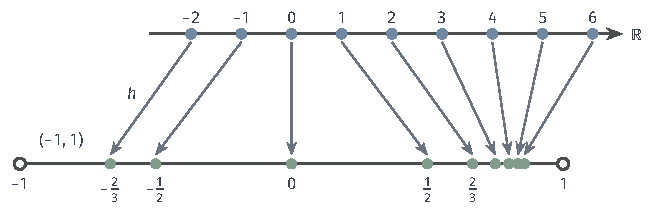
\includegraphics[width=110.659mm]{figures/04-spaces-measures-and-geometry/01-topology-and-metric/tikz/mmap-homeo-line/figure.pdf}
  \caption{同胚$h(x)=x/(1+\lvert x\rvert)$把$\mathbb R$上的整数点（上方，蓝）映到开区间$(-1,1)$内（下方，绿）。上方点列相邻距离恒为$1$，不是柯西列；像点$1-1/n$是柯西列，但极限$1$不在开区间内。}
  \label{fig:mmap-homeo-line}
\end{BookInlineFigure}

$\mathbb R$完备，$(-1,1)$不完备：$y_n=1-1/n$是$(-1,1)$中的柯西列，极限$1$不在其中。用$h^{-1}$搬回实轴，
\[
 h^{-1}(y_n)=\frac{1-1/n}{1/n}=n-1,
\]
相邻两项相距$1$，不是柯西列。同胚把一个柯西列变成了非柯西列，所以柯西性不是拓扑性质，完备性也不是。同样，$(-1,1)$有界、全有界，$\mathbb R$两者都不是，所以有界性与全有界性也不被同胚保持。

换一个角度，同一个集合也可以配上拓扑相同、完备性不同的度量。在$\mathbb R$上令
\[
 d_h(x,y)=\lvert h(x)-h(y)\rvert.
\]
$h$是单射，所以$d_h$是度量；$h:(\mathbb R,d_h)\to(-1,1)$是满射等距映射，所以$(\mathbb R,d_h)$不完备，其中$x_n=n-1$是柯西列而无极限。

另一方面，$h$是通常拓扑下的同胚，$d_h$的开集恰是通常的开集。这就是第~\ref{chap:metric-spaces}章预告的、与通常度量拓扑相同却不完备的度量。

在紧致度量空间之间，这种差别不会出现：紧致蕴含完备且全有界，而紧致是拓扑性质，所以与紧致度量空间同胚的度量空间也完备、全有界。差别只出现在非紧空间中，那里完备性依赖于“无穷远处”的距离怎样度量。

\subsection{同一集合上的度量等价}
\label{sec:mmap-metric-equivalence}

设$d$与$d'$是同一集合$X$上的两个度量。比较它们相当于研究恒等映射$\operatorname{id}:(X,d)\to(X,d')$及其逆满足什么条件。按要求由弱到强，有三种“等价”。

\begin{definition}[度量的三种等价]
\label{def:mmap-metric-equivalence}
设$d,d'$是$X$上的度量。
\begin{enumerate}
\item 若$d$与$d'$诱导相同的开集，即$\operatorname{id}$双向连续，称它们\term{拓扑等价}（topologically equivalent）；
\item 若$\operatorname{id}:(X,d)\to(X,d')$与其逆都均匀连续，称它们\term{一致等价}（uniformly equivalent）；
\item 若存在常数$0<c\leq C$，使对所有$x,y$有
\begin{equation}
 c\,d(x,y)\leq d'(x,y)\leq C\,d(x,y),
 \label{eq:mmap-strong-equivalence}
\end{equation}
即$\operatorname{id}$双向Lipschitz连续，称它们\term{强等价}（strongly equivalent）。
\end{enumerate}
\end{definition}

由Lipschitz连续蕴含均匀连续、均匀连续蕴含连续，强等价蕴含一致等价，一致等价蕴含拓扑等价。三个层次分别保留不同的信息，表~\ref{tab:mmap-metric-equivalence}是一份汇总，下面逐一解释。

\begin{BookInlineTable}
  \centering
  \caption{同一集合上三种度量等价保留的信息}
  \label{tab:mmap-metric-equivalence}
  \begin{tabular}{lll}
    \toprule
    等价层次 & 保留的性质 & 不保留的性质 \\
    \midrule
    拓扑等价 & 收敛点列、紧致、可分 & 柯西列、完备 \\
    一致等价 & 另加柯西列、完备、全有界 & 有界性 \\
    强等价 & 另加有界集、误差尺度 & 常数$c,C$的具体值 \\
    \bottomrule
  \end{tabular}
\end{BookInlineTable}

拓扑等价保留一切拓扑性质。按序列判据，它等价于两个度量下收敛的点列及其极限完全相同，所以紧致、可分以及映射的连续性都不因换用另一个度量而改变。它不保留柯西列：上一小节的$\lvert\cdot\rvert$与$d_h$拓扑等价，但前者完备、后者不完备。

一致等价还保留柯西列与完备性。均匀连续映射把柯西列送到柯西列，恒等映射双向均匀连续，两个度量下的柯西列就相同，而收敛点列本来就相同，所以一个完备当且仅当另一个完备。

它还保留全有界性。给定$\varepsilon$，由$\operatorname{id}:(X,d)\to(X,d')$的均匀连续性取$\delta$，则
\[
 B_d(x,\delta)\subseteq B_{d'}(x,\varepsilon),
\]
$d$下半径$\delta$的有限覆盖就是$d'$下半径$\varepsilon$的覆盖；反方向同理。

一致等价却不保留有界性。$\mathbb R$上的$\lvert x-y\rvert$与$\min\{\lvert x-y\rvert,1\}$在小于$1$的尺度上完全一致，对$\varepsilon<1$取$\delta=\varepsilon$，就得到双向均匀连续。但后者下整个$\mathbb R$有界，而前者下$\mathbb R$无界，所以不存在$c>0$使$\min\{\lvert x-y\rvert,1\}\geq c\lvert x-y\rvert$对所有$x,y$成立。

强等价进一步比较误差的尺度。由式~\eqref{eq:mmap-strong-equivalence}，
\begin{equation}
 B_d(x,r/C)\subseteq B_{d'}(x,r)\subseteq B_d(x,r/c),
 \label{eq:mmap-ball-sandwich}
\end{equation}
所以两个度量下的有界集相同，覆盖数也只差一个尺度因子：
\[
 N^{d'}(C\varepsilon,A)\leq N^{d}(\varepsilon,A),
\]
其中上标表示所用的度量。

$\mathbb R^n$上的$\rho_\infty$与$d_2$是最常见的例子，它们满足
\[
 \rho_\infty(\bm x,\bm y)\leq d_2(\bm x,\bm y)\leq\sqrt n\,\rho_\infty(\bm x,\bm y).
\]

取$n=2$，$d=d_2$，$d'=\rho_\infty$，则$c=1/\sqrt2$，$C=1$。把$r=1$代入式~\eqref{eq:mmap-ball-sandwich}，得
\[
 B_{d_2}(\bm x,1)\subseteq B_{\rho_\infty}(\bm x,1)\subseteq B_{d_2}(\bm x,\sqrt2).
\]
图~\ref{fig:mmap-balls}画出的就是这三个集合：圆盘、外切正方形，以及外接圆盘。

\begin{BookInlineFigure}
  \centering
  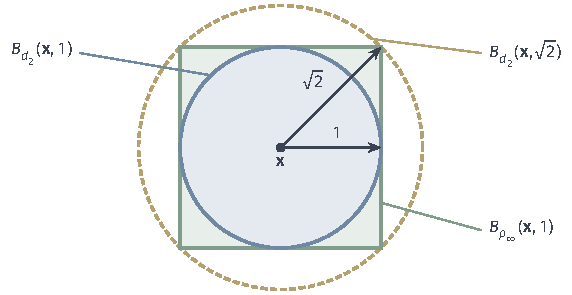
\includegraphics[width=96.852mm]{figures/04-spaces-measures-and-geometry/01-topology-and-metric/tikz/mmap-balls/figure.pdf}
  \caption{$\mathbb R^2$上强等价的两个度量。蓝色圆盘是$d_2$的单位球，绿色正方形是$\rho_\infty$的单位球，黄色虚线圆是$d_2$的半径$\sqrt2$的球。正方形夹在两个圆盘之间，比例由常数$c=1/\sqrt2$，$C=1$决定。}
  \label{fig:mmap-balls}
\end{BookInlineFigure}

卷二证明了有限维空间上任意两个范数诱导的度量都强等价，所以在有限维空间中说“收敛”“有界”“完备”无需指明范数；估计误差时则要记得常数$c,C$可能依赖于维数。这一点在无限维时不再成立，第~\ref{chap:function-normed-spaces}章将看到同一函数空间上不等价的范数。

文献中“等价度量”有时指拓扑等价，有时指强等价。本书遇到这一说法时会写明是哪一种，或直接写出所要求的映射条件。

\section{稠密子集上的映射延拓}
\label{sec:mmap-extension}

只在稠密子集上知道一个映射的值，是常见的情形：先在有理数上定义一个运算，再希望把它推广到全体实数；或者只在有限精度的网格上做过测量，希望确定一个连续量。设$D\subseteq X$稠密，$f:D\to Y$已知。对$x\in X\setminus D$，自然的办法是取$D$中趋于$x$的点列$d_n$，把$f(d_n)$的极限定义为新值。这要求两件事：像点列确实有极限，并且换一个逼近列不会得到不同的结果。本节说明，目标空间完备保证前者，均匀连续保证后者，并且延拓后保留原来的误差控制。

\subsection{延拓的构造}
\label{sec:mmap-extension-construction}

我们先给出定理，再逐步说明每个条件在构造中的作用。

\begin{theorem}[均匀连续映射的延拓]
\label{thm:mmap-extension}
设$D$是度量空间$X$的稠密子集，$Y$是完备度量空间，$f:D\to Y$均匀连续。则存在唯一的连续映射$F:X\to Y$，使$F|_D=f$。
\end{theorem}

\begin{proof}
定义。对$x\in X$，由稠密性和第~\ref{chap:metric-spaces}章的闭包序列判据，取$d_n\in D$使$d_n\to x$。收敛点列是柯西列，均匀连续映射把柯西列送到柯西列，所以$(f(d_n))$是$Y$中的柯西列，由$Y$完备收敛。令$F(x)=\lim_nf(d_n)$。

与逼近列无关。设另有$d_n'\in D$趋于$x$。把两列交替排成新点列$d_1,d_1',d_2,d_2',\ldots$，它仍趋于$x$，于是它的像也是柯西列并收敛到某个$z$。$(f(d_n))$与$(f(d_n'))$都是这个像点列的子列，因而都趋于$z$。所以$F(x)$不依赖于逼近列的选择。

延拓。若$x\in D$，可以取常值逼近列$d_n=x$，得$F(x)=f(x)$。

唯一性。设$G:X\to Y$连续且$G|_D=f$。对$x\in X$及趋于$x$的$d_n\in D$，由序列判据$G(x)=\lim G(d_n)=\lim f(d_n)=F(x)$。$F$本身的连续性在下一小节与误差控制一起证明。
\end{proof}

唯一性的论证只用到$D$稠密与$G$连续，不需要$Y$完备或$f$均匀连续：两个连续映射若在稠密子集上相同，就处处相同。存在性则两个条件都要用，缺一个都会失败。

缺少目标空间的完备性时，像点列可能没有极限。取$X=\mathbb R$、$D=\mathbb Q$、$Y=\mathbb Q$，$f$为$\mathbb Q$上的恒等映射，它是等距映射，当然均匀连续。若有连续延拓$F:\mathbb R\to\mathbb Q$，沿$\sqrt2$的有理截断$q_n$应有$F(\sqrt2)=\lim q_n=\sqrt2$，而$\sqrt2\notin\mathbb Q$。完备性要求作用在目标空间上，定义域$X$完备与否无关紧要。

缺少均匀连续时，不同的逼近列可能给出不同的极限。在$D=\mathbb Q\cap[0,1]$上令$f(q)=0$（$q<1/\sqrt2$）、$f(q)=1$（$q>1/\sqrt2$）。$1/\sqrt2$不是有理数，所以$f$在$D$的每一点附近都是常值，因而连续；但从左、右两侧逼近$1/\sqrt2$的有理数列，像分别恒为$0$与$1$，没有连续延拓到$[0,1]$。这正说明了$f$不均匀连续：两侧的点可以任意接近，函数值却始终相差$1$。

\subsection{延拓后的误差控制}
\label{sec:mmap-extension-error}

延拓不仅存在，还继承原映射在$D$上的误差控制，阈值与常数都不变坏。

\begin{theorem}[延拓保持均匀连续与Lipschitz常数]
\label{thm:mmap-extension-control}
在定理~\ref{thm:mmap-extension}的条件下，设$\varepsilon,\delta>0$满足：$d_1,d_2\in D$且$d(d_1,d_2)<\delta$时$d(f(d_1),f(d_2))<\varepsilon$。则$x,x'\in X$且$d(x,x')<\delta$时$d(F(x),F(x'))\leq\varepsilon$。特别地，$F$均匀连续；若$f$以$L$为Lipschitz常数，则$F$也以$L$为Lipschitz常数。
\end{theorem}

\begin{proof}
取$d_n\to x$，$d_n'\to x'$，$d_n,d_n'\in D$。由三角不等式，$d(d_n,d_n')\to d(x,x')<\delta$，所以$n$充分大时$d(d_n,d_n')<\delta$，从而$d(f(d_n),f(d_n'))<\varepsilon$。令$n\to\infty$，由距离的连续性得$d(F(x),F(x'))\leq\varepsilon$。对任意$\varepsilon$，用$\varepsilon/2$对应的$\delta$，就得到$F$的均匀连续性，特别地$F$连续。

若对$D$中所有点都有$d(f(d_1),f(d_2))\leq L\,d(d_1,d_2)$，则对每个$n$有$d(f(d_n),f(d_n'))\leq L\,d(d_n,d_n')$，两边取极限得$d(F(x),F(x'))\leq L\,d(x,x')$。
\end{proof}

由这两个定理，哪些函数可以由稠密观测唯一确定，答案很清楚。在有理数上给定的函数若在每个有界区间上均匀连续，就唯一地确定了实轴上的连续函数：在每个$[-M,M]$上分别延拓，由唯一性，不同区间上的延拓在公共部分一致；例如多项式$p(q)$在$\mathbb Q\cap[-M,M]$上Lipschitz连续，延拓结果就是同一个多项式在实轴上的取值。反过来，若只知道目标函数连续，在有理点上的值就足以确定它；若函数可以不连续，有理点上的值什么也确定不了，例如在有理点取$0$、在无理点任意取值的函数。

延拓定理还完成了第~\ref{chap:metric-spaces}章留下的一步：完备化在等距意义下唯一。

\begin{theorem}[完备化的唯一性]
\label{thm:mmap-completion-unique}
设$\iota:X\to\hat X$与$j:X\to\tilde X$都是保持距离的映射，$\hat X,\tilde X$完备，像$\iota(X)$与$j(X)$分别稠密。则存在满射等距映射$\Phi:\hat X\to\tilde X$，使$\Phi\circ\iota=j$。
\end{theorem}

\begin{proof}
在稠密子集$\iota(X)$上定义$\phi(\iota(x))=j(x)$，它保持距离，因而是Lipschitz常数为$1$的均匀连续映射。$\tilde X$完备，由定理~\ref{thm:mmap-extension}，$\phi$延拓为连续映射$\Phi:\hat X\to\tilde X$。对$\xi,\eta\in\hat X$，取$\iota(x_n)\to\xi$，$\iota(y_n)\to\eta$，则
\begin{equation*}
\begin{aligned}
d(\Phi(\xi),\Phi(\eta))&=\lim d(j(x_n),j(y_n))=\lim d(x_n,y_n)\\
&=\lim d(\iota(x_n),\iota(y_n))=d(\xi,\eta),
\end{aligned}
\end{equation*}
所以$\Phi$保持距离。像$\Phi(\hat X)$与完备空间$\hat X$等距，因而完备，在$\tilde X$中是闭集；它又包含稠密集$j(X)$，所以等于$\tilde X$。
\end{proof}

\section{压缩映射}
\label{sec:mmap-contraction}

许多方程可以写成$x=T(x)$的形式，满足它的点称为$T$的\term{不动点}（fixed point）。最朴素的解法是反复代入：任取初值$x^{(0)}$，计算$x^{(1)}=T(x^{(0)})$，$x^{(2)}=T(x^{(1)})$，……，希望迭代列趋于一个解。例如解$x=(x+2)/3$时，从$0$出发得到$2/3,\ 8/9,\ 26/27,\ldots$，看上去趋于$1$。本节说明这种做法什么时候一定成功：$T$把空间映回自身，按统一的比例缩小距离，并且空间完备。它把Lipschitz误差控制与完备性结合起来，不仅给出解的存在与唯一，还给出迭代误差的界。

\begin{definition}[压缩映射]
\label{def:mmap-contraction}
设$(X,d)$是度量空间。映射$T:X\to X$若存在常数$q\in[0,1)$，使对所有$x,y\in X$有
\begin{equation}
d(T(x),T(y))\leq q\,d(x,y),
\label{eq:mmap-contraction}
\end{equation}
则称$T$为\term{压缩映射}（contraction mapping），$q$称为\term{压缩常数}（contraction constant）。
\end{definition}

定义中有三个要求，后面的反例会逐一说明它们都不能去掉：$T$的值仍在$X$中，所以迭代可以无限进行；同一个$q<1$对所有点对有效，而不只是每对点各自缩小距离；$q<1$严格成立。压缩映射以$q$为Lipschitz常数，因而连续。

\begin{theorem}[压缩映射定理]
\label{thm:mmap-banach-fixed-point}
设$(X,d)$是非空完备度量空间，$T:X\to X$是压缩常数为$q$的压缩映射。则$T$有唯一的不动点$x^\ast$；对任意初值$x^{(0)}\in X$，迭代$x^{(k+1)}=T(x^{(k)})$收敛于$x^\ast$，并且对$k\geq1$，
\begin{equation}
d(x^{(k)},x^\ast)\leq\frac{q^k}{1-q}\,d(x^{(1)},x^{(0)}),\qquad
d(x^{(k)},x^\ast)\leq\frac q{1-q}\,d(x^{(k)},x^{(k-1)}).
\label{eq:mmap-contraction-error-bounds}
\end{equation}
\end{theorem}

下面三个小节依次证明迭代收敛于不动点、不动点唯一，以及两个误差界。

\subsection{迭代收敛}
\label{sec:mmap-iteration-convergence}

先估计相邻两次迭代之差。由$x^{(k+1)}=T(x^{(k)})$与$x^{(k)}=T(x^{(k-1)})$，压缩条件给出$d(x^{(k+1)},x^{(k)})\leq q\,d(x^{(k)},x^{(k-1)})$，反复使用得
\begin{equation*}
d(x^{(k+1)},x^{(k)})\leq q^k\,d(x^{(1)},x^{(0)}).
\end{equation*}
每一步的移动量按几何级数缩小。

相邻项接近还不够，柯西列要求任意两个后项接近。对$m>k$，沿途使用三角不等式，再对几何级数求和：
\begin{equation}
d(x^{(m)},x^{(k)})\leq\sum_{j=k}^{m-1}d(x^{(j+1)},x^{(j)})\leq\sum_{j=k}^{m-1}q^j\,d(x^{(1)},x^{(0)})\leq\frac{q^k}{1-q}\,d(x^{(1)},x^{(0)}).
\label{eq:mmap-contraction-cauchy}
\end{equation}
右端与$m$无关，并且$q<1$时随$k\to\infty$趋于零，所以$(x^{(k)})$是柯西列。

由$X$完备，迭代列收敛到某个$x^\ast\in X$。再用$T$的连续性：$T(x^\ast)=\lim_kT(x^{(k)})=\lim_kx^{(k+1)}=x^\ast$，所以$x^\ast$是不动点。这里三个要求各司其职：$T(X)\subseteq X$使迭代列有定义，统一的$q<1$使几何级数收敛，完备性使柯西列有极限。

\subsection{不动点的唯一性}
\label{sec:mmap-fixed-point-uniqueness}

设$x^\ast$与$y^\ast$都是不动点。由压缩条件，
\begin{equation*}
d(x^\ast,y^\ast)=d(T(x^\ast),T(y^\ast))\leq q\,d(x^\ast,y^\ast),
\end{equation*}
即$(1-q)\,d(x^\ast,y^\ast)\leq0$。由$q<1$得$d(x^\ast,y^\ast)=0$，两者相同。唯一性只用到$q<1$，不需要完备性：在不完备的空间中压缩映射可能没有不动点，但不会有两个。

结合上一小节，从任何初值出发的迭代都收敛到某个不动点，而不动点只有一个，所以所有迭代都趋于同一个$x^\ast$。也可以直接看出这一点：$d(x^{(k)},x^\ast)=d(T(x^{(k-1)}),T(x^\ast))\leq q\,d(x^{(k-1)},x^\ast)$，所以$d(x^{(k)},x^\ast)\leq q^k\,d(x^{(0)},x^\ast)$。误差每步至少缩小为原来的$q$倍，只是这个式子含有未知的$x^\ast$，不能直接计算。

\subsection{迭代误差界}
\label{sec:mmap-error-bounds}

式\eqref{eq:mmap-contraction-error-bounds}的两个界把未知的误差换成可以计算的量。

第一个界由式\eqref{eq:mmap-contraction-cauchy}令$m\to\infty$得到，因为$d(x^{(m)},x^{(k)})\to d(x^\ast,x^{(k)})$。它只用到初始步长$d(x^{(1)},x^{(0)})$，所以算出第一步后就能预先安排迭代次数：要使误差不超过$\tau$，只需
\begin{equation*}
\frac{q^k}{1-q}\,d(x^{(1)},x^{(0)})\leq\tau,\qquad\text{即}\qquad k\geq\frac{\ln\bigl(\tau(1-q)/d(x^{(1)},x^{(0)})\bigr)}{\ln q}.
\end{equation*}
这样的估计称为\term{先验误差界}（a priori error bound）。

第二个界利用已经算出的最近一步。由三角不等式与压缩条件，
\begin{equation*}
d(x^{(k)},x^\ast)\leq d(x^{(k)},x^{(k+1)})+d(x^{(k+1)},x^\ast)\leq q\,d(x^{(k)},x^{(k-1)})+q\,d(x^{(k)},x^\ast),
\end{equation*}
移项即得$(1-q)\,d(x^{(k)},x^\ast)\leq q\,d(x^{(k)},x^{(k-1)})$。同样的推导对任意点$x$给出$d(x,x^\ast)\leq d(x,T(x))/(1-q)$：一点的残差$d(x,T(x))$越小，它离不动点越近。这样的估计称为\term{后验误差界}（a posteriori error bound），可以作为停止判据：当$q\,d(x^{(k)},x^{(k-1)})/(1-q)\leq\tau$时停止，就保证误差不超过$\tau$。

两个界都依赖压缩常数，因子$1/(1-q)$在$q$接近$1$时很大。例如$q=0.99$时，后验界要求步长小于$\tau/99$才能保证误差小于$\tau$；同时误差每步只缩小$1\%$，收敛很慢。还要注意，后验判据的可靠性来自已知的$q$。不知道映射是否为压缩时，“步长已经很小”本身说明不了什么：调和级数的部分和每步只增加$1/k$，步长趋于零，部分和却趋于无穷。

\subsection{算例与反例}
\label{sec:mmap-contraction-examples}

先在一个可以完全手算的例子上核对定理。

\begin{example}[一次函数的迭代]
\label{ex:mmap-linear-iteration}
在完备空间$\mathbb R$上取$T(x)=(x+2)/3$。$\lvert T(x)-T(y)\rvert=\lvert x-y\rvert/3$，所以$T$是压缩常数$q=1/3$的压缩映射，唯一不动点由$x=(x+2)/3$解得$x^\ast=1$。从$x^{(0)}=0$出发，
\begin{equation*}
x^{(1)}=\tfrac23,\quad x^{(2)}=\tfrac89,\quad x^{(3)}=\tfrac{26}{27},\quad x^{(4)}=\tfrac{80}{81},
\end{equation*}
一般地$x^{(k)}=1-3^{-k}$，因为$1-x^{(k+1)}=(1-x^{(k)})/3$。实际误差是$3^{-k}$。

先验界为$\frac{(1/3)^k}{1-1/3}\cdot\frac23=3^{-k}$。取$k=3$，后验界为$\frac{1/3}{2/3}\bigl(\frac{26}{27}-\frac{24}{27}\bigr)=\frac1{27}$，也等于实际误差$3^{-3}$。两个界在这里都取等号，因为$T$是一次函数，压缩不等式本身就是等式。要使误差不超过$10^{-6}$，需要$3^{-k}\leq10^{-6}$，即$k\geq6\ln10/\ln3\approx12.6$，取$k=13$。
\end{example}

下面的例子说明定理的每个条件都不能省略。

缺少完备性时，极限可能不在空间中。在$X=(0,1)$上取$T(x)=x/2$，它把$X$映入自身，压缩常数为$1/2$。迭代$x^{(k)}=2^{-k}x^{(0)}$是柯西列，在$\mathbb R$中趋于$0$，但$0\notin X$；方程$x=x/2$在$\mathbb R$中只有解$0$，所以$T$在$X$中没有不动点。

压缩常数等于$1$时，距离不缩小，几何级数也不再收敛。在完备空间$\mathbb R$上取$T(x)=x+1$，有$\lvert T(x)-T(y)\rvert=\lvert x-y\rvert$，迭代每步移动$1$，不是柯西列；$x=x+1$无解。即使每对点的距离都严格缩小，只要没有统一的$q<1$，结论也可能失败。在完备空间$[1,\infty)$上取$T(x)=x+1/x$，它把$[1,\infty)$映入自身；由中值定理，$\lvert T(x)-T(y)\rvert=(1-1/\xi^2)\lvert x-y\rvert<\lvert x-y\rvert$（$x\neq y$，$\xi$介于两者之间），但$1-1/\xi^2$可以任意接近$1$。方程$x=x+1/x$无解，迭代列单调增加趋于无穷。

$T$必须把空间映回自身。在完备空间$[0,1/2]$上，$T(x)=(x+2)/3$仍满足压缩不等式，但$T(0)=2/3\notin[0,1/2]$，迭代离开了所给的空间，唯一的不动点$1$也不在其中。实际使用压缩映射定理时，常常先找一个被$T$映入自身的闭集，再在这个闭集上验证压缩条件；闭集作为完备空间的子空间仍完备。

压缩映射定理在其他地方多次出现。线性方程组的定常迭代$\bm x^{(k+1)}=\bm G\bm x^{(k)}+\bm c$中，若迭代矩阵在某个诱导范数下满足$\lVert\bm G\rVert<1$，迭代映射就是压缩常数为$\lVert\bm G\rVert$的压缩映射，这类格式的收敛分析可参考\BookChapterRef{chap:stationary-iterations}{卷二“定常迭代法”章}；常微分方程初值问题的Picard迭代在连续函数空间中验证压缩条件，由此得到解的存在唯一，可参考\BookChapterRef{chap:ordinary-differential-equations}{卷六“常微分方程与初值问题”章}。那里所用的完备函数空间，正是第~\ref{sec:mmap-uniform-cauchy}小节的有界连续函数空间。

\section{本章小结}
\label{sec:mmap-summary}

本章开头的问题是：输入的误差经过映射后变成多大的输出误差，近似映射的极限保留什么性质，反复代入何时能求出方程的解。第一层回答是连续性本身。在度量空间之间，第~\ref{chap:topological-spaces}章的开集原像定义等价于逐点的$\varepsilon$-$\delta$保证，也等价于保持收敛点列的极限；连续性保证原像保持开闭，不保证像保持开闭；序列判据的反向依赖每点有可数个球作邻域基，一般拓扑空间中只有正方向成立。

第二层回答是统一的误差控制。均匀连续要求阈值与位置无关，从而把柯西列送到柯西列；Lipschitz连续进一步要求输出误差不超过输入误差的固定倍数，多步计算的放大倍数至多相乘。三种条件依次加强，$x^2$与$\sqrt x$分别说明连续不必均匀连续、均匀连续不必Lipschitz连续。紧定义域上连续自动均匀连续，等度连续族自动一致等度连续，但紧性不提供Lipschitz常数。

第三层回答涉及映射列与映射族。逐点收敛允许达到精度所需的序号随输入改变，一致收敛则要求统一的序号；一致极限保持连续，而这只需目标空间是度量空间。目标空间完备时，一致柯西列必有一致极限，由此有界映射空间与有界连续映射空间在一致度量下完备，这是后面函数空间完备性的共同依据。等度连续要求全族共用阈值，为第~\ref{chap:function-class-covers}章的紧性判据作准备。

最后，映射条件与空间的性质配合使用。等距映射保留一切度量性质；同胚只保留拓扑性质，实轴与开区间说明完备、有界都不是拓扑性质；同一集合上的度量按拓扑等价、一致等价、强等价分别保留收敛与紧性、柯西列与完备性、有界性与误差尺度。完备目标空间中，稠密子集上的均匀连续映射唯一地延拓到全空间，并保留阈值与Lipschitz常数，由此完备化在等距意义下唯一。压缩映射定理把统一的压缩常数与完备性结合起来：几何级数给出柯西列，完备性给出极限，连续性证明它是不动点，先验与后验误差界则告诉我们何时可以停止迭代。

